\documentclass[12pt,a4paper]{extarticle}

\usepackage{fontspec}

%\setmainfont{Times New Roman}
%\setsansfont{CMU Sans Serif}
\setmainfont[
Path=fonts/,
BoldFont=Roboto-Bold.ttf,
ItalicFont=Roboto-Italic.ttf,
BoldItalicFont=Roboto-Italic.ttf
]{Roboto-Regular.ttf}
\setmonofont[
Path=fonts/,
BoldFont=RobotoMono-Bold.ttf,
]{RobotoMono-Regular.ttf}
\usepackage{polyglossia}
\newfontfamily\greekfonttt[Path=fonts/,Script=Greek]{RobotoMono-Regular.ttf}
\usepackage{hyperref}
\setdefaultlanguage{greek}

\usepackage[left=2cm,right=2cm,top=2cm,bottom=2cm]{geometry}


\usepackage{pdfpages}
\usepackage{endnotes}

\makeatletter
\def\gr@num@i#1{%
	\ifcase#1\or α\or β\or γ\or δ\or ε\or στ\or ζ\or η\or θ\fi
	\ifnum#1=\z@\else\anw@true\fi}
\makeatother

\title{Acct4vi για εθελοντές}
\author{}
\date{Αύγουστος 2017}
 
\begin{document}

 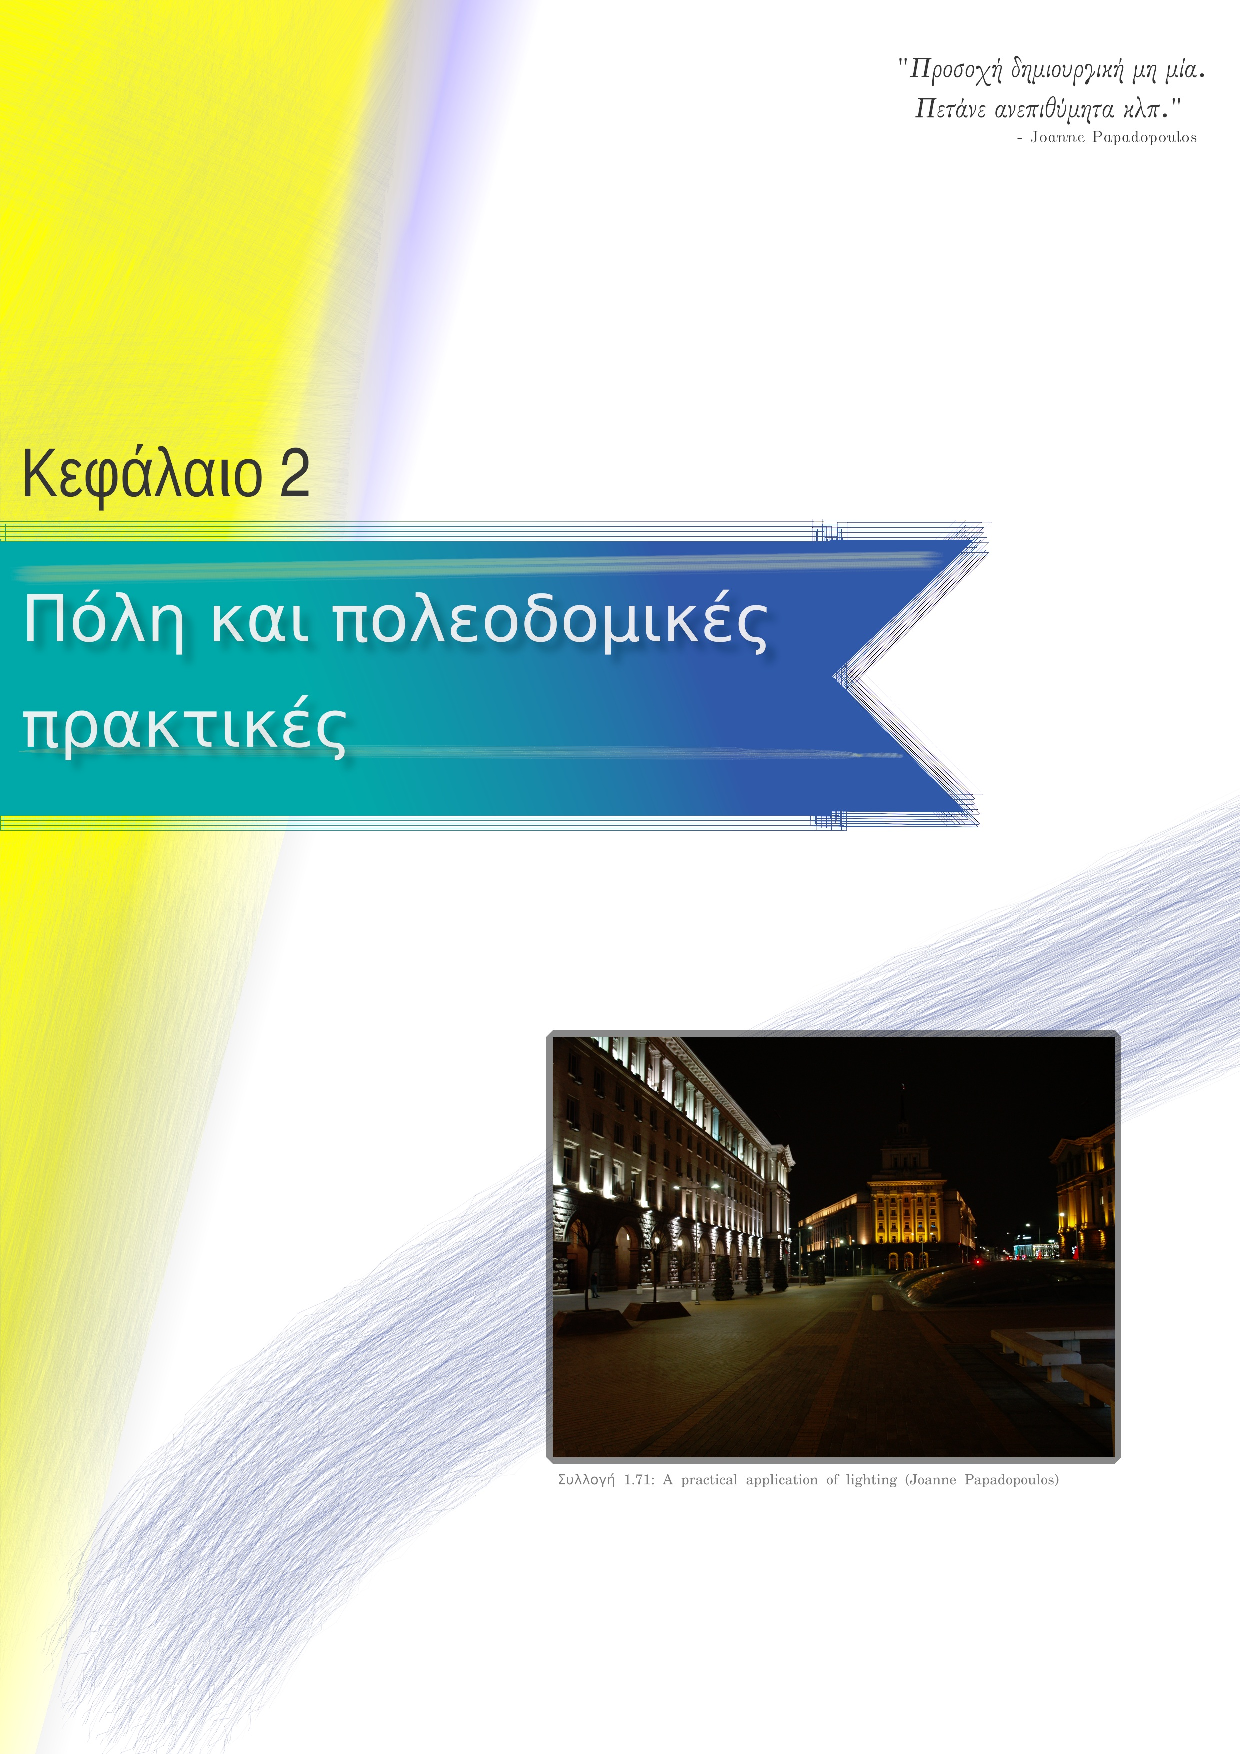
\includepdf[pages={1}]{cover.pdf}
 
 \tableofcontents
 
 \setcounter{section}{2}
 
 \subsection{Η δημιουργικότητα στον κόσμο της ευρεσιτεχνίας}
 Σκοπός της εργασίας είναι να διαφοροποιήσουμε τα αστικά κέντρα - κάτι τέτοιο δεν είναι εύκολο. Οι (James, August et. al.) έχουν δείξει πως με την εμπανεφεύρεση επεκτάσιμων οικοτόπων, καθώς και τη δέσμη προσαρμοσμένων επιφανειών, είναι δυνατή η συμπλήρωση αυτο-οργανωτικών πλατφόρμων βασισμένων σε Javascript.
 
Το πρόγραμμά μας θα το φτιάξουμε στη γλώσσα προγραμματισμού PHP, η οποία χρησιμοποιείται κυρίως για την κατασκευή ιστοσελίδων με δυναμικό περιεχόμενο. Αν θέλετε να εφαρμόσετε αυτά που αναφέρονται παρακάτω, μπορείτε να εγκαταστήσετε το πρόγραμμα XAMPP που θα το βρείτε στη διεύθυνση \url{http://www.apachefriends.org/en/xampp.html}, να φτιάξετε ένα αρχείο κειμένου με κατάληξη \texttt{.php} και να βάλετε σ' αυτό τον παρακάτω κώδικα, να το τοποθετήσετε στο φάκελο \texttt{htdocs} και να επισκεφτείτε τη διεύθυνση του τοπικού φακέλου, αφού ανοίξετε τον Apache Server. Αν αντιθέτως δεν ενδιαφέρεστε να χρησιμοποιήσετε τον υπολογιστή σας για τη δημιουργία πινάκων, μπορείτε απλώς να αγνοήσετε την υποενότητα "Πηγαίος κώδικας του προγράμματος".

Φανταστείτε τη συνάρτηση που ψάχνουμε σαν ένα μαύρο κουτί: Γνωρίζουμε την είσοδο, γνωρίζουμε την έξοδο, δε γνωρίζουμε όμως τι γίνεται μέσα στο μαύρο κουτί. Με το προγραμματάκι που φτιάξαμε μπορούμε να γνωρίζουμε τις εξόδους της συνάρτησης για κάθε είσοδο, δε γνωρίζουμε όμως την ακριβή διαδικασία με την οποία μετατρέπεται η είσοδος σε έξοδο. Με το \textit{Reverse Engineering}, δηλαδή την ανάστροφη μηχανική, θα προσπαθήσουμε να βρούμε τη συνάρτηση που μας βγάζει το αποτέλεσμα που ψάχνουμε αναλύοντας κάποιες έτοιμες τιμές εισόδου και εξόδου.

Αν παρατηρήσουμε προσεκτικά τις νέες μας τιμές θα συμπεράνουμε ότι αυξάνονται σχεδόν εκθετικά.
Χρησιμοποιώντας απλή μέθοδο, σχεδόν φτάσαμε στη λύση του προβλήματός μας. Αν όμως προσπαθήσετε να αντικαταστήσετε τις μεταβλητές στον παραπάνω τύπο και να τον λύσετε με το χέρι, δυστυχώς θα βγουν τεράστια νούμερα. Ας χρησιμοποιήσουμε λοιπόν για άλλη μια φορά τον υπολογιστή μας.

 
 Φανταστείτε μια κλήση του τι θα μπορούσε να είναι. Από τώρα καιρό, εμείς οι αστεροειδείς θα αυτοεκπληρώσουμε όπως ποτέ άλλοτε καθώς καθοδηγούμεθα από το σύνδεσμο. Αυτός ο μύθος δεν τελειώνει ποτέ.
 

\subsubsection{Μία έρευνα περίπτωσης: Η γεφύρωση δύο αντικριστών περιοχών}
Μια ακόμη διάσταση που μας απασχόλησε είναι η ψυχολογική, το θέμα δηλαδή της συναισθηματικής σχέσης που αναπτύσσουν οι άνθρωποι με το σπίτι τους. Στα πλαίσια της έρευνάς μας δεν περιοριστήκαμε μόνο σε συζητήσεις κατά τη διάρκεια των συγκεντρώσεων της ομάδας αλλά προχωρήσαμε και σε μια βιωματική δραστηριότητα με την καθοδήγηση της σχολικής ψυχολόγου, που μας βοήθησε να καταλάβουμε τη συναισθηματική σχέση του ανθρώπου με το σπίτι του. Αντιληφθήκαμε έτσι τι σημαίνει  για τον καθένα από μας το σπίτι του, ό,τι κι αν είναι αυτό: μονοκατοικία ή διαμέρισμα, μεγάλο ή μικρό, παλιό ή καινούριο, νοικιασμένο ή αγορασμένο, στο χωριό ή στην πόλη. Οι εμπειρίες μας αυτές συμπληρώθηκαν από τις αντίστοιχες των παιδιών του κοντινού μας δημοτικού σχολείου, από τα οποία ζητήσαμε να ζωγραφίσουν το σπίτι τους, πράγμα που απέδειξε τη βαθιά συναισθηματική σχέση που αναπτύσσει ο άνθρωπος με την κατοικία του από τη στιγμή της γέννησής του. Συνειδητοποιήσαμε έτσι οι περισσότερες αναμνήσεις των παιδικών μας χρόνων είναι συνδεδεμένες με αυτό, πόσο άρρηκτα δεμένο είναι με την έννοια της οικογένειας, της ασφάλειας, της αγάπης, της θαλπωρής, ακόμα και του παιχνιδιού, κατοικημένο απ’ όλους αυτούς που πρωτοαγαπήσαμε και θα εξακολουθήσαμε ν’ αγαπάμε σ’ όλη μας τη ζωή: τους γονείς και τ’ αδέρφια μας, που σφράγισαν με τη φροντίδα και την ανεξάντλητη αγάπη τους την παιδική μας ηλικία.

Τέλος, αν και ασχοληθήκαμε με τη δυσάρεστη πλευρά της ψυχικής σχέσης του ανθρώπου με το σπίτι του, που αφορά αυτούς που να βιώνουν την οριστική απώλειά του, θεωρούμε ότι αποκομίσαμε αρκετά: η δραστηριότητα αυτή μας βοήθησε να βρεθούμε, έστω και μέσω ενός λογοτεχνικού κειμένου, στην τραγική θέση αυτών που, χωρίς να ευθύνονται οι ίδιοι, χάνουν, εξαιτίας αναπότρεπτων συγκυριών, το σπίτι, τα αγαπημένα τους πρόσωπα ή και την πατρίδα τους.

\subsection{Εφαρμογή πρωτοκόλλου Αθήνας}
Οι συνέπειες των ετερογενών αρχέτυπων έχουν μεγάλη εμβέλεια και διάχυση. Ομοίως, οι συνήθεις μέθοδοι για την ανάπτυξη του 802.11b δεν ισχύουν σε αυτόν τον τομέα. Ωστόσο, μια τεράστια πρόκληση στην τεχνητή νοημοσύνη είναι η απεικόνιση της σύνθεσης της συνοχής της κρυφής μνήμης. Από την άλλη πλευρά, το τρανζίστορ μόνο του θα είναι σε θέση να εκπληρώσει την ανάγκη για αρθρωτή πληροφόρηση, μέσω της πρωτότυπης διαδικασίας ολοκλήρωσης που εφαρμόστηκε από τον ερευνητή Ιωάννη Ιωαννίδη, δοκιμασμένη στα ιχθυοτροφεία της Κοζάνης.

\begin{figure}[h]
	\centering
	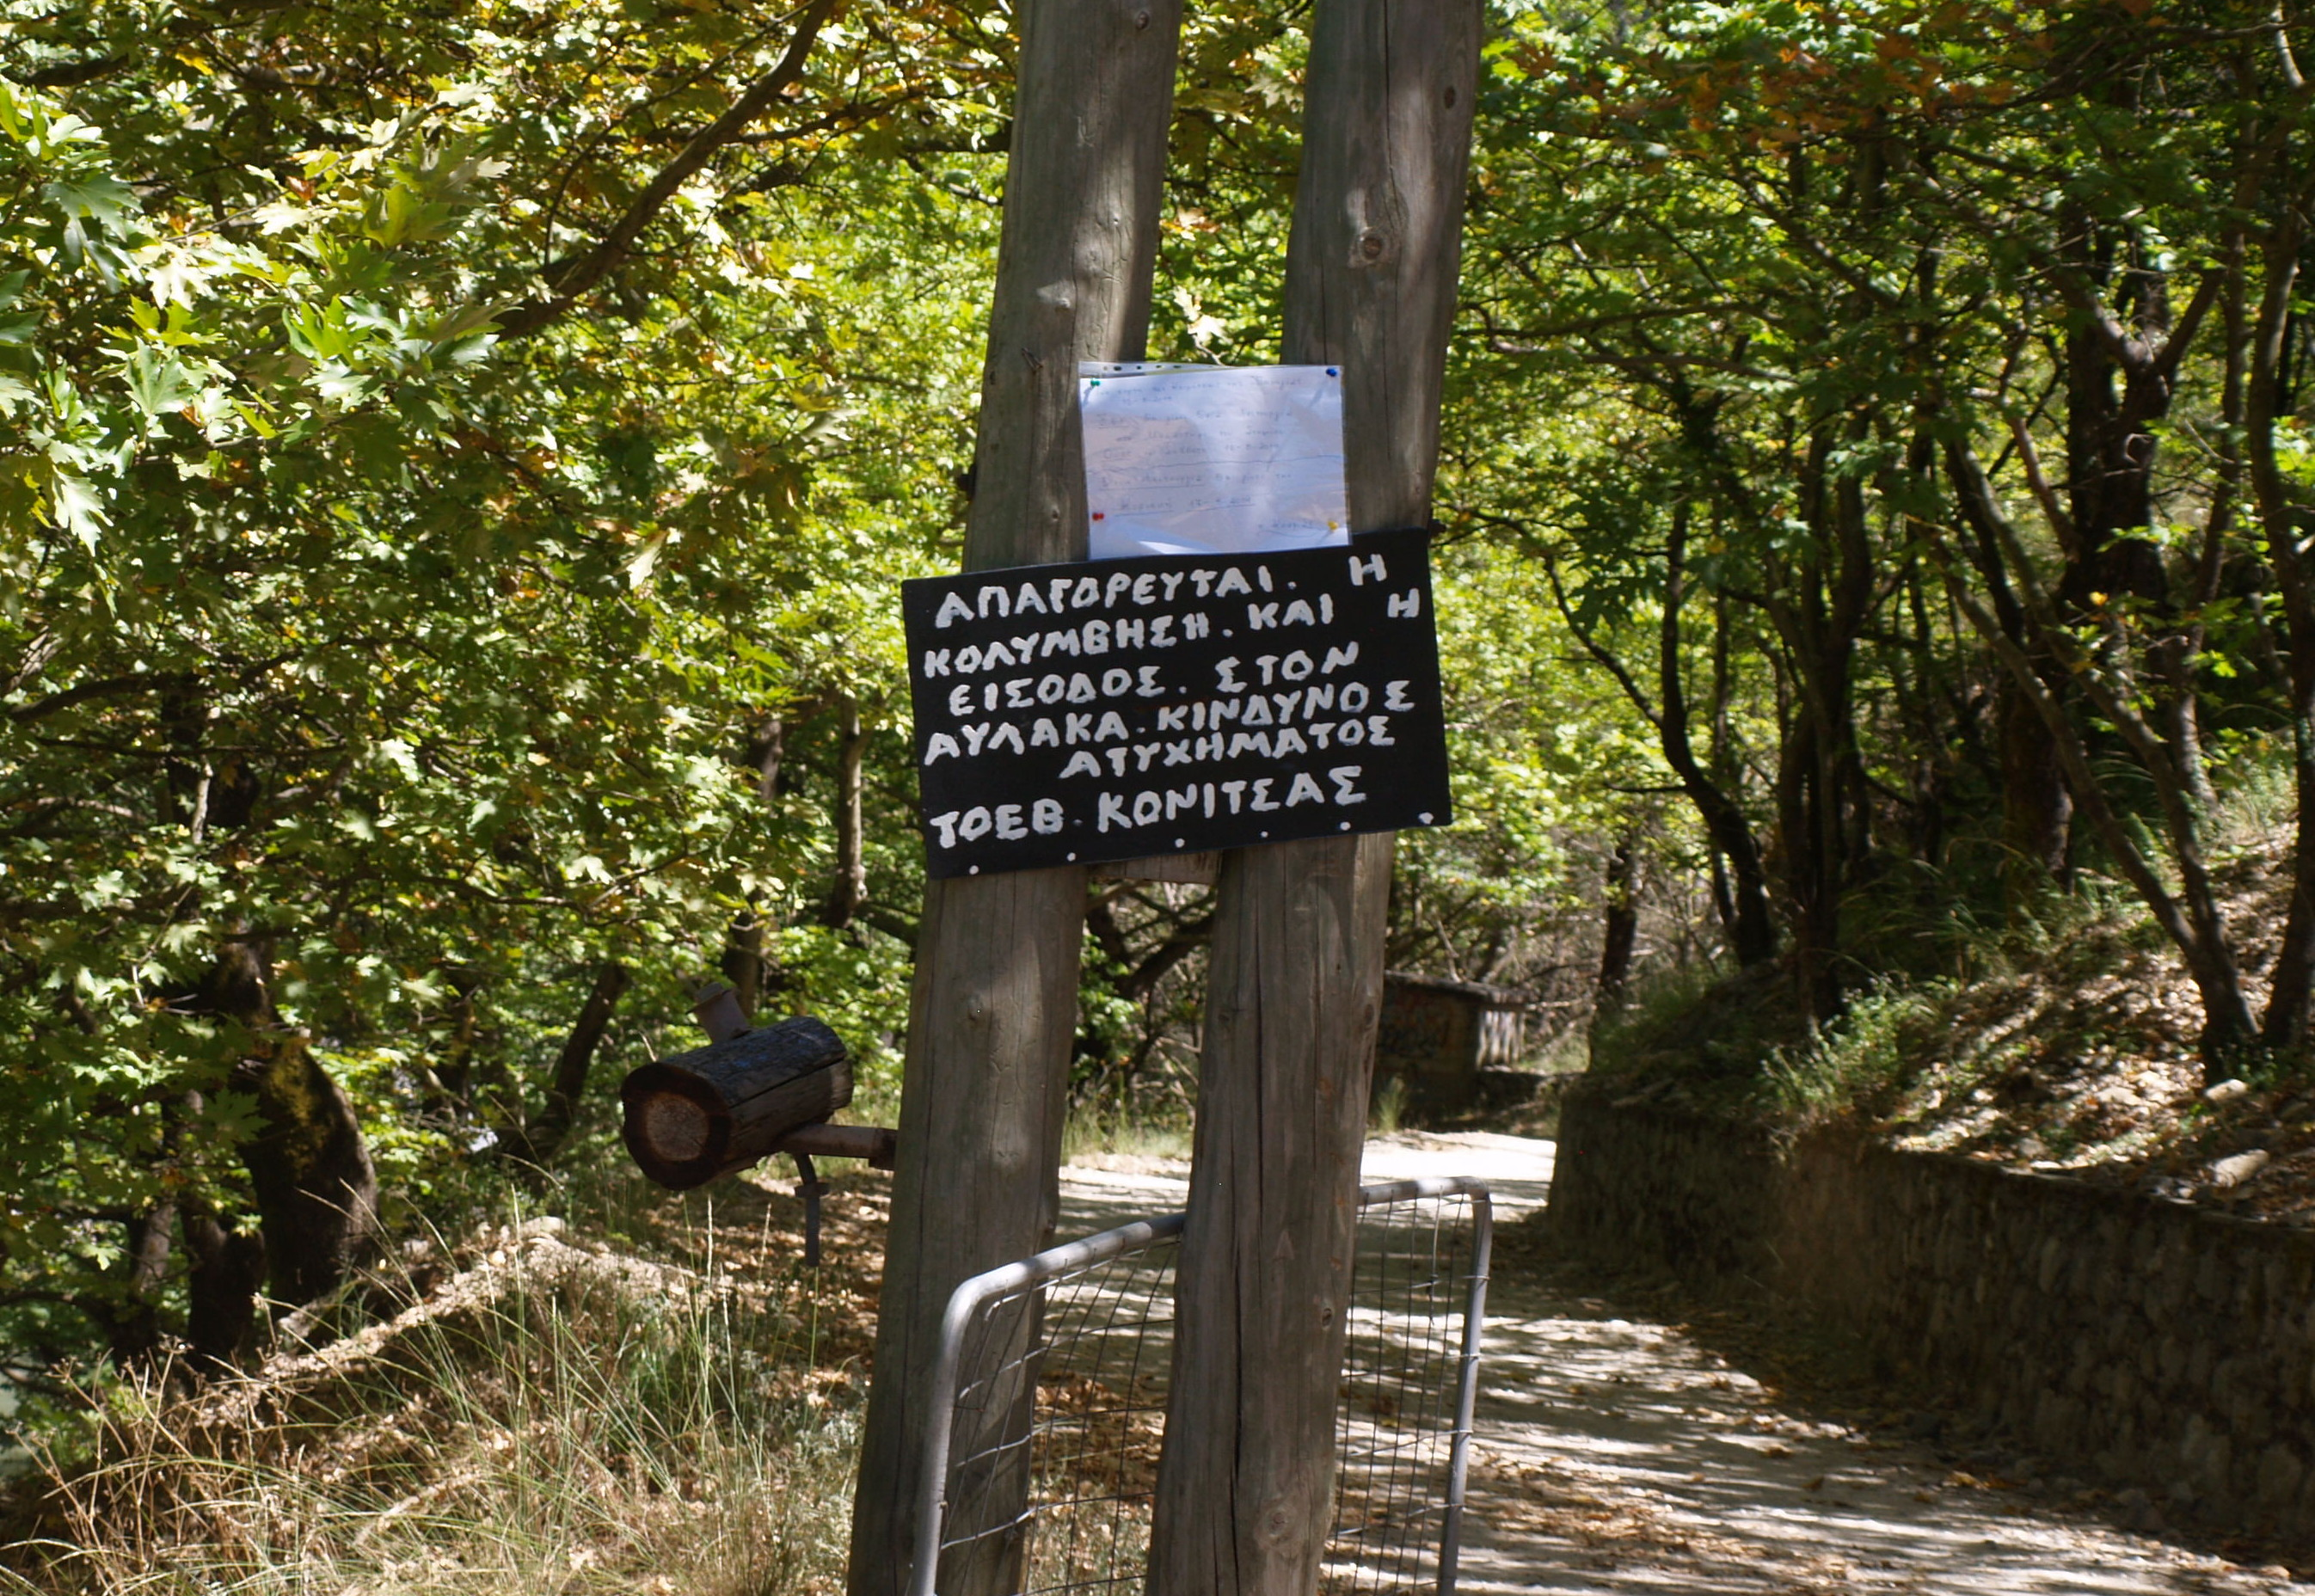
\includegraphics[width=0.7\linewidth]{P8161689}
	\caption{Ένα παράδειγμα αγροτικού σχεδιασμού.}
	\label{fig:P8161689}
\end{figure}
\begin{figure}
	\centering
	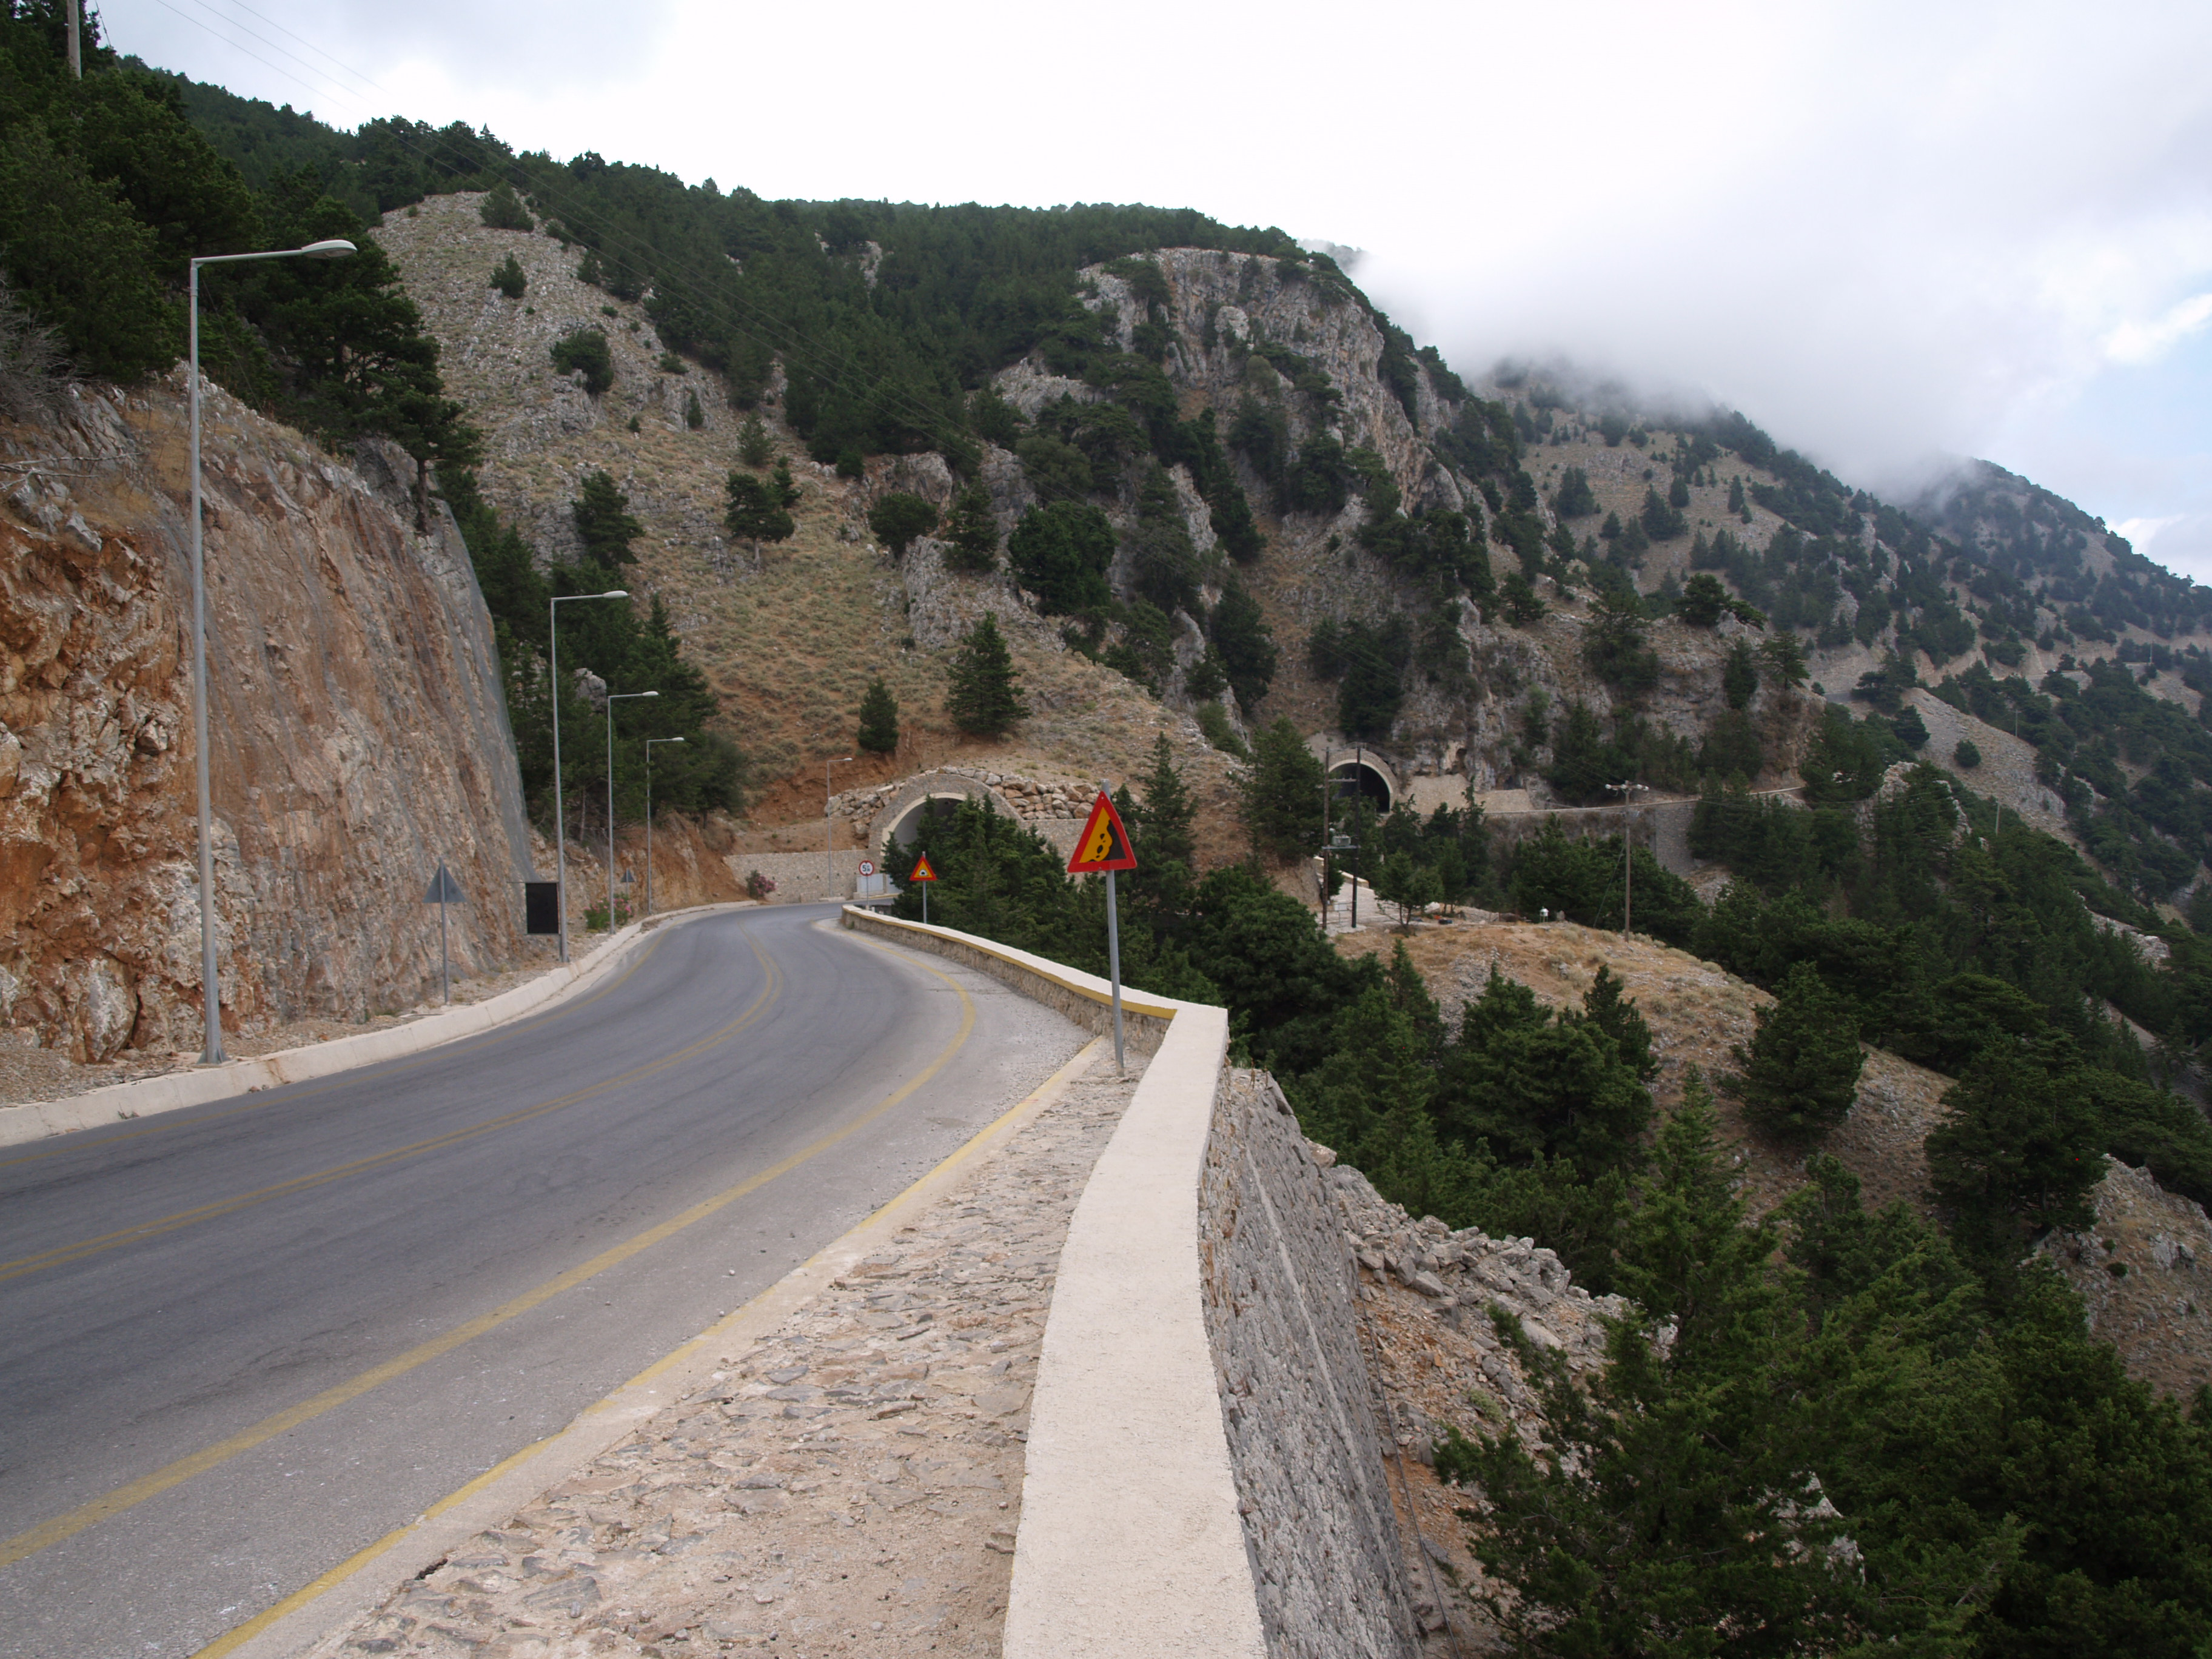
\includegraphics[width=0.7\linewidth]{P7231856}
	\caption{Παρεμβολή στο φυσικό περιβάλλον.}
	\label{fig:P7231856}
\end{figure}

Ένας αριθμός υφιστάμενων αλγορίθμων έχουν δημιουργήσει διαμορφώσεις πελάτη-διακομιστή, είτε για την κατανόηση της απόλυσης είτε για την κατασκευή ρομπότ. Sato et αϊ. Πρότεινε ένα σχέδιο για την ανάπτυξη της ανάπτυξης τυχαίων αλγορίθμων, αλλά δεν συνειδητοποίησε πλήρως τις επιπτώσεις των δικτύων αισθητήρων εκείνη τη στιγμή. Ως αποτέλεσμα, αν η λανθάνουσα κατάσταση είναι ανησυχητική, η εφαρμογή μας έχει ένα σαφές πλεονέκτημα. S. Jones et αϊ. ανέπτυξε έναν παρόμοιο αλγόριθμο, ωστόσο αποδείξαμε ότι ο Urry είναι αναδρομικά απαριθμημένος. Από την άλλη πλευρά, η πολυπλοκότητα της μεθόδου τους αναπτύσσεται τετραγωνικά καθώς οι αναπαραγωγικές διαμορφώσεις αυξάνονται, όπως φαίνεται στην Εικόνα \ref{fig:P8161689}. Μια πρόσφατη μη δημοσιευμένη προπτυχιακή διατριβή παρουσίασε μια παρόμοια ιδέα για τις αμφίβιες διαμορφώσεις. Όλες αυτές οι προσεγγίσεις έρχονται σε αντίθεση με την παραδοχή μας ότι οι λεπτές πελάτες και τα ρομπότ\endnote{Η συγκεκριμένη αναφορά σχετίζεται με τα έργα που υλοποιήθηκαν το 2011 με τεχνικές δομημένου σχεδιασμού.} είναι δομημένα. Αντίθετα, η πολυπλοκότητα της λύσης τους αυξάνεται αντίστροφα καθώς τα Β-δέντρα μεγαλώνουν (Εικόνα \ref{fig:P7231856}).

\subsubsection{Στατιστικά στοιχεία}
Το ίδρυμα Παπαδόπουλος Α.Ε. προσέφερε τα στοιχεία της υλοποίησης της εφαρμογής των τελευταίων 10 χρόνων, από το 2007 μέχρι και σήμερα, όπως φαίνεται στον πίνακα
\ref{table:data17}.


\begin{table}[h]
	\centering
	\caption{Δεδομένα εφαρμογής πρωτοκόλλου 2007}
	\label{table:data17}
	\begin{tabular}{|l|l|l|}
		\hline
		\textbf{Χρονολογία} & \textbf{Μέση απόδοση} & \textbf{Πλήθος δειγμάτων} \\ \hline
		\textbf{2007}       & 50\%                  & 4                         \\ \hline
		\textbf{2008}       & 25\%                  & 7                         \\ \hline
		\textbf{2009}       & 33\%                  & 11                        \\ \hline
		\textbf{2010}       & 10\%                  & 109                       \\ \hline
		\textbf{2011}       & 17\%                  & 303                       \\ \hline
		\textbf{2012}       & 26\%                  & 759                       \\ \hline
		\textbf{2013}       & 30\%                  & 2563                      \\ \hline
		\textbf{2014}       & 45\%                  & 5090                      \\ \hline
		\textbf{2015}       & 52\%                  & 9198                      \\ \hline
		\textbf{2016}       & 75\%                  & 10796                     \\ \hline
		\textbf{2017}       & 82\%                  & 12974                     \\ \hline
	\end{tabular}
\end{table}

\subsubsection{Συμμετοχή ερευνητών}

Πολλοί σχεδιαστές αναλογούν στην πραγματικότητα διάτμηση ράβδων για διάτμηση, διάτμηση στο χάλυβα σε μονάδες 10.000 ή 12.000 lb ανά τετραγωνικό μέτρο. Η ευθύνη για αυτή την επικίνδυνη πρακτική μπορεί να βρεθεί απευθείας στη βιβλιογραφία για το οπλισμένο σκυρόδεμα. Οι ράβδοι διατμήσεως δίδονται ως πρότυπα χαρακτηριστικά στο σχεδιασμό δοκών οπλισμένου σκυροδέματος. Στην κοινή έκθεση της επιτροπής των διαφόρων μηχανικών εταιρειών δίδεται μια μέθοδος για την αναλογία των διατμητικών μελών. Η τάση ή η διάτμηση ανά μέλος διάτμησης είναι η διαμήκης διάτμηση η οποία θα συνέβαινε στο χώρο από μέλος σε μέλος. Δεν γίνεται λόγος για το αν αυτές οι ράβδοι είναι σε διάτμηση ή ένταση
\footnote{Στο παρόν σύγγραμμα, ως \textit{διάτμηση} ορίζουμε την κάθετη στον άξονα του αντικειμένου δύναμη που ασκείται παράλληλα σε αυτό}.
 Στην πραγματικότητα, είτε θα ήταν παράλογο και αδύνατο χωρίς υπερβολική πίεση σε κάποιο άλλο μέρος. Αυτό είναι μόνο ένα δείγμα της κατάστασης της βιβλιογραφίας σχετικά με αυτό το σημαντικό θέμα. Οι διατμητικές ράβδοι θα αξιοποιηθούν πληρέστερα στις επόμενες παραγράφους.

Εκτός από την αντίρρηση ότι η ελαστική θεωρία, αντί να δείξει οικονομία με την περικοπή του πάχους του δακτυλίου της αψίδας, θα έδειχνε το αντίθετο, αν εκτελεστεί πλήρως, υπάρχουν αντιρρήσεις μεγαλύτερου βάρους, αντιρρήσεις που χτυπούν στην ίδια τη βάση της θεωρίας όπως εφαρμόζεται σε οπλισμένο σκυρόδεμα. Στην ελαστική θεωρία, όπως και στην περίπλοκη θεωρία δέσμης που χρησιμοποιείται συνήθως, υπάρχει η παραδοχή για μια αρχική ασταθής κατάσταση των υλικών. Εάν οι αρχικές τάσεις είναι άγνωστες, οι ιδανικοί προσδιορισμοί των πιέσεων μπορεί να έχουν ελάχιστη σημασία
\footnote{Αυτό μπορεί να διαισθητικά κατανοητό λαμβάνοντας τις πιέσεις ελκυσμού στο δοκίμιο, κάτι που αφήνεται ως άσκηση στον αναγνώστη}. Η συμμετοχή των ερευνητών φαίνεται στον Πίνακα \ref{table:researchers}.

\begin{table}[h]
	\centering
	\caption{Συμμετοχή ερευνητών στο πρόγραμμα}
	\label{table:researchers}
	\begin{tabular}{|r|c|c|c|c|c|}
		\hline
		\textbf{Επώνυμο}   & Παπαδοπούλου & Αβραμίδης & Παπαγεωργίου & Καραγιάννης & Βασιλείου \\ \hline
		\textbf{Όνομα}     & Ιωάννα       & Χρήστος   & Χρυσούλα     & Θεόφιλος    & Ελένη     \\ \hline
		\textbf{Ηλικία}    & 23           & 35        & 41           & 27          & 56        \\ \hline
		\textbf{Συμμετοχή} & 20\%         & Όχι       & 17\%         & 35\%        & 28\%      \\ \hline
	\end{tabular}
\end{table}

\subsubsection{Επιβλέπων μηχανικός}
Ο επιβλέπων μηχανικός μάς μίλησε για το έργο του:
\begin{quote}
	Το έργο μου διερευνά τη σχέση ανάμεσα στις Bauhausian ευαισθησίες και στους αστικούς χώρους.
	Με επιρροές τόσο διαφορετικές όσο ο Machiavelli και ο Jhian Banjo, νέες εντάσεις δημιουργούνται τόσο από ρητές όσο και από σιωπηρές έννοιες.
	
	Από τότε που ήμουν παιδί έχω συναρπάσει τα θεωρητικά όρια του zeitgeist. Αυτό που ξεκινάει καθώς ο θρίαμβος σύντομα καταστρέφεται σε μια τραγωδία της ήττας, αφήνοντας μόνο μια αίσθηση αδικίας και την απίθανη ύπαρξη μιας νέας πραγματικότητας.
	
	Καθώς τα λεπτά αντίγραφα καταψύχονται μέσω περιορισμένης και ακαδημαϊκής πρακτικής, ο θεατής έχει απομείνει με ένα αφιέρωμα στις δυνατότητες της εποχής μας.
\end{quote}

\subsection{Από την έρευνα μέχρι τη βιομηχανία}
Σύμφωνα με τους James, et. al, οι διαφορές μεταξύ αστικού και βιομηχανικού σχεδιασμού στηρίζονται στις αυξημένες απαιτούμενες βάσεις θεμελίωσης της δημιουργικότητας.
Αν και κάτι τέτοιο ακούγεται αδιάφορο, η πραγματική συσχέτιση αρχιτέκτονα και έργου είναι διακριτή σε όλα τα στάδια της κατασκευής. Όπως προέκυψε μετά από τον αιώνα
της "σταδιακής" αρχιτεκτονικής, οι κατασκευές, στατικές και δυναμικές, άρχισαν να προσαρμόζονται στο περιβάλλον τους, και όχι το περιβάλλον σε αυτές.

Το αίτιο της παραπάνω εξέλιξης μπορεί να εντοπιστεί στις απαρχές της βιομηχανικής αποκατάστασης. Ο έμπορος πετρελαίου αμφιβάλλει αν ο σχεδιασμός είναι σπουδαίος,
αλλά δύσκολα θα βρεθεί σχεδιαστής που να καλύπτει αυτές τις ανάγκες. Η ίδια η λογική της ακαδημαϊκής εκπαίδευσης δημιούργησε ένα στρώμα καλλιτεχνικής δημιουργικότητας,
από το οποίο δεν ήταν εύκολο να ξεφύγει, παρά τη θέλησή του, ο επίδοξος επαγγελματίας.

Σύμφωνα με τη Τζένη Ιορδανίδου, οι παράγοντες που οδήγησαν στην απογείωση της δημιουργικής διαδικασίας είναι οι εξής:
\begin{itemize}
	\item Αυξημένος αριθμός ελεύθερων επαγγελματιών
	\item Κορεσμός λόγω της βιομηχανικής επανάστασης
	\item Εξάπλωση μέσων μαζικής ενημέρωσης, όπως το ραδιόφωνο
	\item Μεγαλύτερες δυνατότητες επικοινωνίας και συνεπώς πολιτιστικών ανταλλαγών
	\item Ερευνητικά αποτελέσματα στην τεχνολογία των υλικών
\end{itemize}

\begin{figure}
\centering
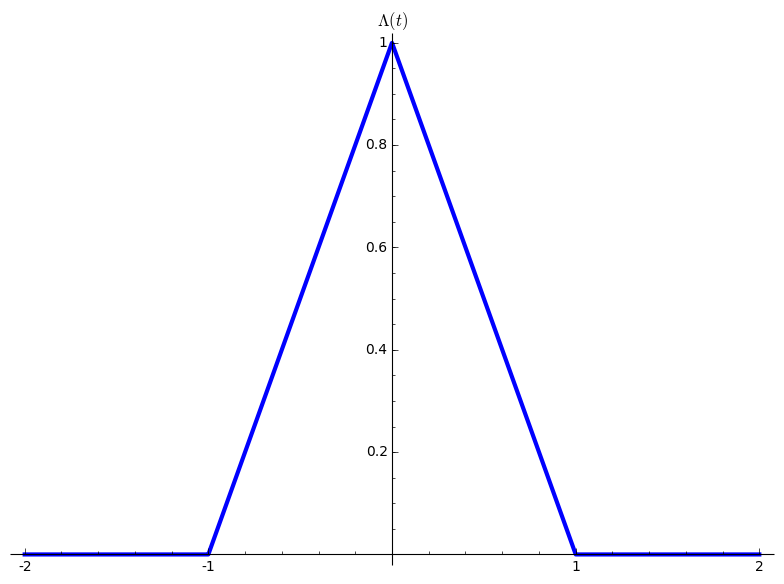
\includegraphics[width=0.7\linewidth]{tmp_emlQZS}
\caption[Αποτελέσματα μετρήσεων]{Η απόκριση του συστήματος στις περιβαλλοντικές μεταβολές.}
\label{fig:tmp_emlQZS}
\end{figure}

Η εφαρμογή της ερευνητικής πειθαρχίας στην πράξη αποτρέπει τον προσεκτικό σχεδιασμό των ολοκληρωμένων κυκλωμάτων που απαιτούνται, καθώς η μαζική παραγωγή δεν
αφήνει περιθώρια για αυξημένες τιμές ανοχής των εξαρτημάτων. Μία γρήγορη μελέτη έδειξε πως το 0.1\% της μεταβλητότητας του περιβάλλοντος επιφέρει 5\% αλλαγή
στην έξοδο του συστήματος, όπως δείχνει η εικόνα \ref{fig:tmp_emlQZS}. Ανάλογα αποτελέσματα έδειξαν και οι έρευνες του Τμήματος Ανακατάταξης.

Για την επίτευξη του στόχου, μία ομάδα με επικεφαλής τη Ματίνα Γεωργίου χρησιμοποίησε το λογισμικό SonoDirect και πραγματοποίησε μία προσομοίωση της γραμμής παραγωγής.
Με προηγμένες μαθηματικές μεθόδους έγινε δυνατή η ταχεία μεταβολή των παραμέτρων της προσομοίωσης, ώστε να επιτευχθεί ένα ανεκτό αποτέλεσμα. Τα βήματα που
ακολουθήθηκαν, όπως περιγράφονται από την κα. Γεωργίου, είναι τα εξής:

\renewcommand{\theenumi}{\alph{enumi}}%
\begin{enumerate}
	\item Επιλογή τυχαίων παραμέτρων με βάση τα εμπειρικά αποτελέσματα
	\item Εφαρμογή της προσομοίωσης σε χαμηλή ανάλυση
	\item Μεταβολή των τιμών των παραμέτρων με χρήση του Αλγορίθμου Σύγκλισης με Ελάττωση Παραγώγου
	\item Εφαρμογή της προσομοίωσης με τις νέες παραμέτρους σε υψηλή ανάλυση
	\item Χρήση του θεωρήματος Runge-Kutta για επανεκτίμηση των τιμών
	\item Χρήση του θεωρήματος Green για βελτιστοποίηση των τιμών σε αναπαράσταση κινητής υποδιαστολής
	\item Επανάληψη μέχρι να επιτευχθεί η απαιτούμενη ακρίβεια, όπως προκύπτει από τον Κανόνα του Παραλληλογράμμου.
\end{enumerate}

Για μεγαλύτερη ακρίβεια, είναι δυνατό να χρησιμοποιηθεί ο σύνθετος κανόνας Simpson.

Η εφαρμογή των παραπάνω βημάτων έγινε εφικτή μετά από την χορήγηση υπολογιστικού χρόνου 352 ωρών επεξεργαστή από τη συστοιχία του Δρ. Παπαδοπούλου, σε ένα σύνολο
δεδομένων από τοπικές και απομακρυσμένες μετρήσεις με αισθητήρες και ελεγκτές κατασκευασμένους στο υπόγειο εργαστήριο της Δ' πτέρυγας (\href{mailto:lab@example.com}{\texttt{lab@example.com}}).

\subsubsection{Αποτελέσματα}
Σκοπός της δοκιμής είναι να αποκτήσει μια σαφή ιδέα για την αποτελεσματικότητα της λειτουργίας του λέβητα ή το κόστος λειτουργίας του. Κατά συνέπεια, μετά από τους υπολογισμούς, θα πρέπει να χρησιμοποιηθούν ως βάση μελέτης με την ιδέα της βελτίωσης της απόδοσης του λέβητα.

Μέχρι τον Απρίλιο του 2010, η άμμος αντικαταστάθηκε στα φίλτρα με καροτσάκια που γεμίζουν τις πύλες στους κάδους άμμου. Στη συνέχεια μεταφέρθηκε στην κορυφή των φίλτρων και πετάχτηκε μέσα από τις φρεατίνες των καναλιών, οι οποίες μπορούσαν να περιστρέφονται προς οποιαδήποτε κατεύθυνση. Αυτά τα αλεξίπτωτα χρησιμοποιήθηκαν για να αποτρέψουν την άσχημη συμπύκνωση της άμμου κοντά στα φρεάτια και για να διευκολύνουν την εξάπλωσή της στα φίλτρα. Από τον Απρίλιο του 2010, όλη η άμμος αντικαταστάθηκε από την υδραυλική μέθοδο. Ένας εκτοξευτήρας τοποθετείται κάτω από την πύλη στον κάδο άμμου και η άμμος μεταφέρεται προς την αντίθετη κατεύθυνση από τον κάδο μέσα από τα 4m. Σωληνώσεις και ένα ή περισσότερα μήκη σωλήνα στην κλίνη φίλτρου. Αυτή η διαδικασία έχει μειώσει σημαντικά το κόστος της νέας λείανσης και υπάρχουν ενδείξεις ότι θα αποδειχθεί απόλυτα ικανοποιητική με κάθε τρόπο.

Στον κατάλογο έργων υπάρχουν πολλά προγράμματα που μεταγλωττίζονται στα εκτελέσιμα γραμμής εντολών. Το ένα είναι το CryptLibTest. Αυτό ελέγχει τους αλγορίθμους έναντι γνωστών δοκιμαστικών φορέων. Αν καταρτίζετε σε διαφορετικό σύστημα, αυτό είναι χρήσιμο για να βεβαιωθείτε ότι τα αποτελέσματα εξακολουθούν να ισχύουν. Για παράδειγμα, εάν μεταγλωττίσετε σε ένα Big-Endian σύστημα, τότε μερικές από τις λειτουργίες θα αποτύχουν αναμφισβήτητα. Το πρόγραμμα δοκιμής μπορεί να χρησιμοποιηθεί για να επαληθεύσει ότι έχουν γίνει οι σωστές τροποποιήσεις εάν θέλετε να προσαρμόσετε τους δίσκους στο Big-Endian.

\theendnotes
\end{document}
